\task{Декомпозиционный кубизм}
\begin{itemize}

\itA Из восьми одинаковых кубиков сложим кубик $2 \times 2 \times 2$. Его поверхность окажется разделённой на 24 квадрата. Можно ли расставить в эти квадраты числа от 1 до 24 так, чтобы \\
— на каждой грани большого куба сумма чисел была равна 50, \\
— числа на противоположных гранях маленьких кубиков различались на 1?\\
Если можно, то покажите, как. Если нет, то докажие, что нельзя.

\itB Как изменится ответ в предыдущем пункте, если к тому же сумма трёх чисел вокруг каждой из вершин большого кубика должна быть равна 37?

\itC Илья разрезает кубик Рубика $3\times 3\times 3$ на кубики $1\times 1\times 1$. За один раз можно сделать разрез в одной плоскости, при этом перед следующим разрезом можно переставлять в пространстве уже отрезанные части. За сколько разрезаний можно справиться? Объясните, почему за меньшее число нельзя.
\end{itemize}

\vspace{-0.3cm}
\begin{center}
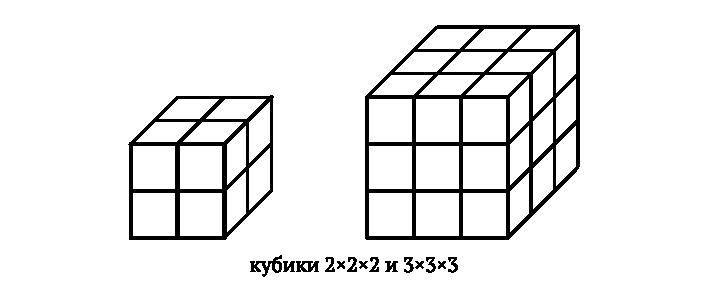
\includegraphics[width=10.5cm]{stats/2017/images/cubes.pdf}
\end{center} \vspace{-0.7cm}